\documentclass{article} 
\usepackage{xcolor} 

%% Page Margins %%
\usepackage{geometry}
\geometry{
    top = 0.75in,
    bottom = 0.75in,
    right = 0.75in,
    left = 0.75in,
}

\usepackage{amsmath}
\usepackage{graphicx}
\usepackage{parskip}

\title{Lab 2: The Design Hierarchy}

\author{\textcolor{blue}{Tyseer Toufiq}}

\begin{document}
\maketitle

\section*{Part I}

\begin{enumerate}
\item If the truth table in Table 2.1 of the handout was given in full, how many rows would it have?

\textcolor{blue}{Since we have 2 selection lines ($s_0$ and $s_1$) and we also have 4 inputs (u,v,w,x) we will have a total of 6 lines to consider. Since each line can be either a 0 or a 1, we have in total $2^6 = 64$ }

\item Export the schematic of the mux4to1 subcircuit as an image and include it in your report.
% TODO

\begin{figure}[ht!]
    \centering
    \includegraphics[width=0.6\textwidth]{part1.png}
    \caption{A schematic of the 4-to-1 multiplexer}
    \label{f:part1}
\end{figure}
\end{enumerate}

\section*{Part II}

\begin{enumerate}
\item Derive seven truth tables, one for each segment of the 7-segment decoder.

\begin{table}[ht!]
\small
\centering
\textcolor{blue}{%
\begin{tabular}{c|c|ccccccc}
$D_{3:0}$ & Character & $S_0$ & $S_1$ & $S_2$ & $S_3$ & $S_4$ & $S_5$ & $S_6$\\
\hline
0000 & 0 & 1 & 1 & 1 & 1 & 1 & 1 & 0 \\
0001 & 1 & 0 & 1 & 1 & 0 & 0 & 0 & 0 \\
0010 & 2 & 1 & 1 & 0 & 1 & 1 & 0 & 1 \\
0011 & 3 & 1 & 1 & 1 & 1 & 0 & 0 & 1 \\
0100 & 4 & 0 & 1 & 1 & 0 & 0 & 1 & 1 \\
0101 & 5 & 1 & 0 & 1 & 1 & 0 & 1 & 1 \\
0110 & 6 & 1 & 0 & 1 & 1 & 1 & 1 & 1 \\
0111 & 7 & 1 & 1 & 1 & 0 & 0 & 0 & 0 \\
1000 & 8 & 1 & 1 & 1 & 1 & 1 & 1 & 1 \\
1001 & 9 & 1 & 1 & 1 & 0 & 0 & 1 & 1 \\
1010 & A & 1 & 1 & 1 & 0 & 1 & 1 & 1 \\
1011 & b & 0 & 0 & 1 & 1 & 1 & 1 & 1 \\
1100 & c & 1 & 0 & 0 & 1 & 1 & 1 & 0 \\
1101 & d & 0 & 1 & 1 & 1 & 1 & 0 & 1 \\
1110 & E & 1 & 0 & 0 & 1 & 1 & 1 & 1 \\
1111 & F & 1 & 0 & 0 & 0 & 1 & 1 & 1 \\
\end{tabular}%
}
\caption{Your Table Caption}
\label{tab:your_table_label}
\end{table}

\item Use Karnaugh maps to write seven Boolean functions for each segment so that they are optimized.


% \textcolor{blue}{
% \begin{align*}
%     S_0 &= (\overline{SW2} \cdot \overline{SW0}) + (\overline{SW3} \cdot SW1) + (SW2 \cdot SW1 ) + (SW3 \cdot \overline{SW0}) + (\overline{SW3} \cdot SW2 \cdot SW0) + (SW3 \cdot \overline{SW2} \cdot \overline{SW1})   \\
%     S_1 &= (\overline{SW3} \cdot \overline{SW2}) + (\overline{SW0} \cdot \overline{SW2}) + 
%     (\overline{SW0} \cdot \overline{SW1} \cdot \overline{SW3}) + (\overline{SW3} \cdot SW1 \cdot SW0) + (SW3 \cdot \overline{SW1} \cdot \overline{SW0}) \\
%     S_2 &= (\overline{SW3} \cdot \overline{SW1}) + (\overline{SW3} \cdot SW0) + (\overline{SW1} \cdot SW0) + (\overline{SW3} \cdot SW2) + (SW3 \cdot \overline{SW2}) \\
%     S_3 &= (\overline{SW3} \cdot \overline{SW2} \cdot \overline{SW0}) + (\overline{SW2} \cdot SW1 \cdot SW0) + (SW2 \cdot \overline{SW1} \cdot SW0) + (SW2 \cdot SW1 \cdot \overline{SW0}) + (SW3 \cdot \overline{SW1} \cdot \overline{SW0})  \\
%     S_4 &= (\overline{SW2} \cdot \overline{SW0}) + (SW1 \cdot \overline{SW0}) + (SW3 \cdot SW1) + (SW3 \cdot SW2) \\
%     S_5 &= (\overline{SW1} \cdot \overline{SW0}) + (SW2 \cdot \overline{SW0}) + (SW3 \cdot \overline{SW2}) + (SW3 \cdot SW1) + (\overline{SW3} \cdot SW2  \cdot \overline{SW1}) \\
%     S_6 &= (\overline{SW2} \cdot SW1) + (SW1 \cdot \overline{SW0}) + (SW3 \cdot \overline{SW2}) + (SW3 \cdot SW0) + (\overline{SW3} \cdot SW2 \cdot \overline{SW1}) \\
% \end{align*}} 

\textcolor{blue}{
\begin{align*}
    S_0 &= (\overline{B} \cdot \overline{D}) + (\overline{A} \cdot C) + (B \cdot C) + (A \cdot \overline{D}) + (\overline{A} \cdot B \cdot D) + (A \cdot \overline{B} \cdot \overline{C})   \\
    S_1 &= (\overline{A} \cdot \overline{B}) + (\overline{D} \cdot \overline{B}) + 
    (\overline{D} \cdot \overline{C} \cdot \overline{A}) + (\overline{A} \cdot C \cdot D) + (A \cdot \overline{C} \cdot D) \\
    S_2 &= (\overline{A} \cdot \overline{C}) + (\overline{A} \cdot D) + (\overline{C} \cdot D) + (\overline{A} \cdot B) + (A \cdot \overline{B}) \\
    S_3 &= (\overline{A} \cdot \overline{B} \cdot \overline{D}) + (\overline{B} \cdot C \cdot D) + (B \cdot \overline{C} \cdot D) + (B \cdot C \cdot \overline{D}) + (A \cdot \overline{C} \cdot \overline{D})  \\
    S_4 &= (\overline{B} \cdot \overline{D}) + (C \cdot \overline{D}) + (A \cdot C) + (A \cdot B) \\
    S_5 &= (\overline{C} \cdot \overline{D}) + (B \cdot \overline{D}) + (A \cdot \overline{B}) + (A \cdot C) + (\overline{A} \cdot B  \cdot \overline{C}) \\
    S_6 &= (\overline{B} \cdot C) + (C \cdot \overline{D}) + (A \cdot \overline{B}) + (A \cdot D) + (\overline{A} \cdot B \cdot \overline{C}) \\
\end{align*}}


\item Use the naming scheme \verb|HEX0|, \verb|HEX1|, ..., \verb|HEX6| for each subcircuit.
    Export each subcircuit schematic as an image and include it in your report.
% TODO

\begin{figure}[ht!]
    \centering
    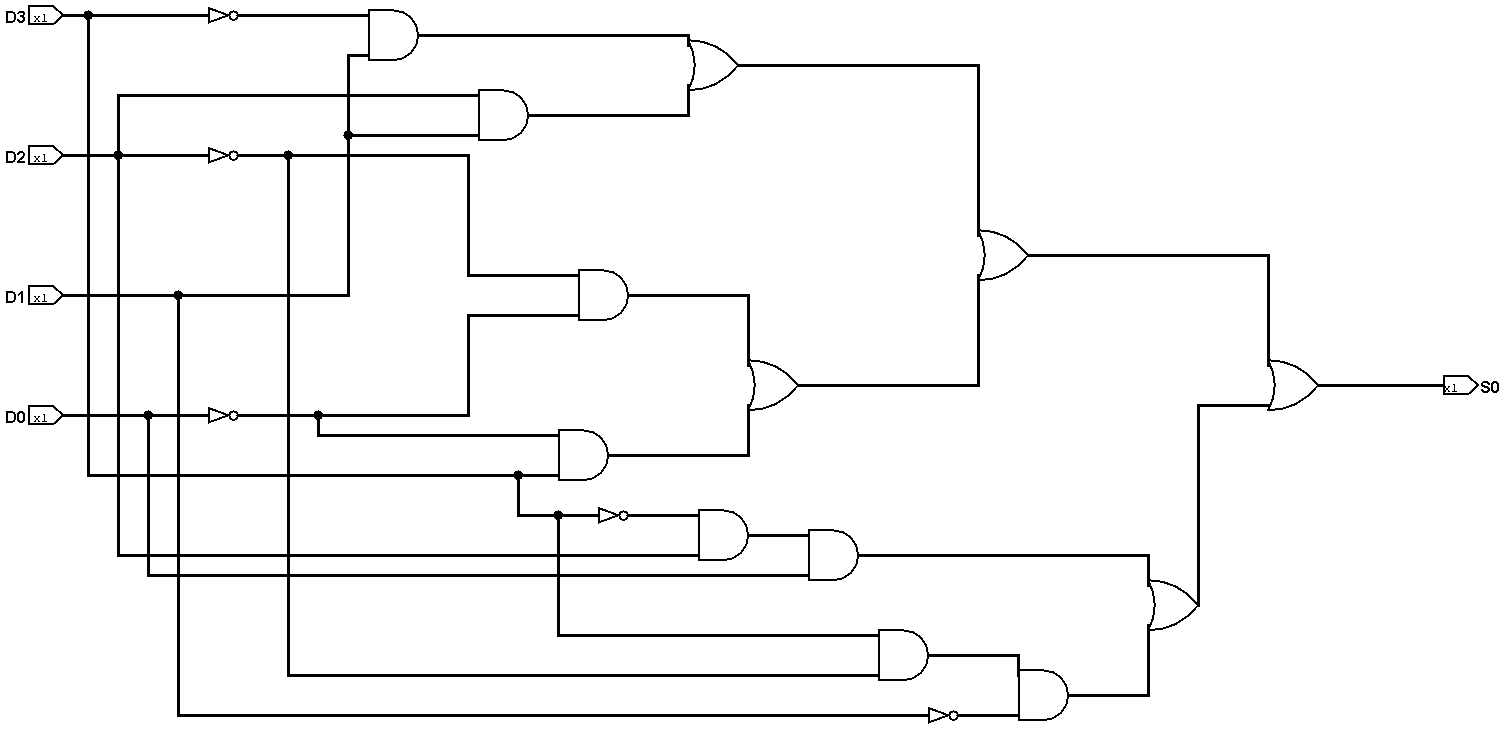
\includegraphics[width=0.7\textwidth]{part2_hex0.png}
    \caption{A schematic of HEX0}
    \label{f:part2_hex0}
\end{figure}

\begin{figure}[ht!]
    \centering
    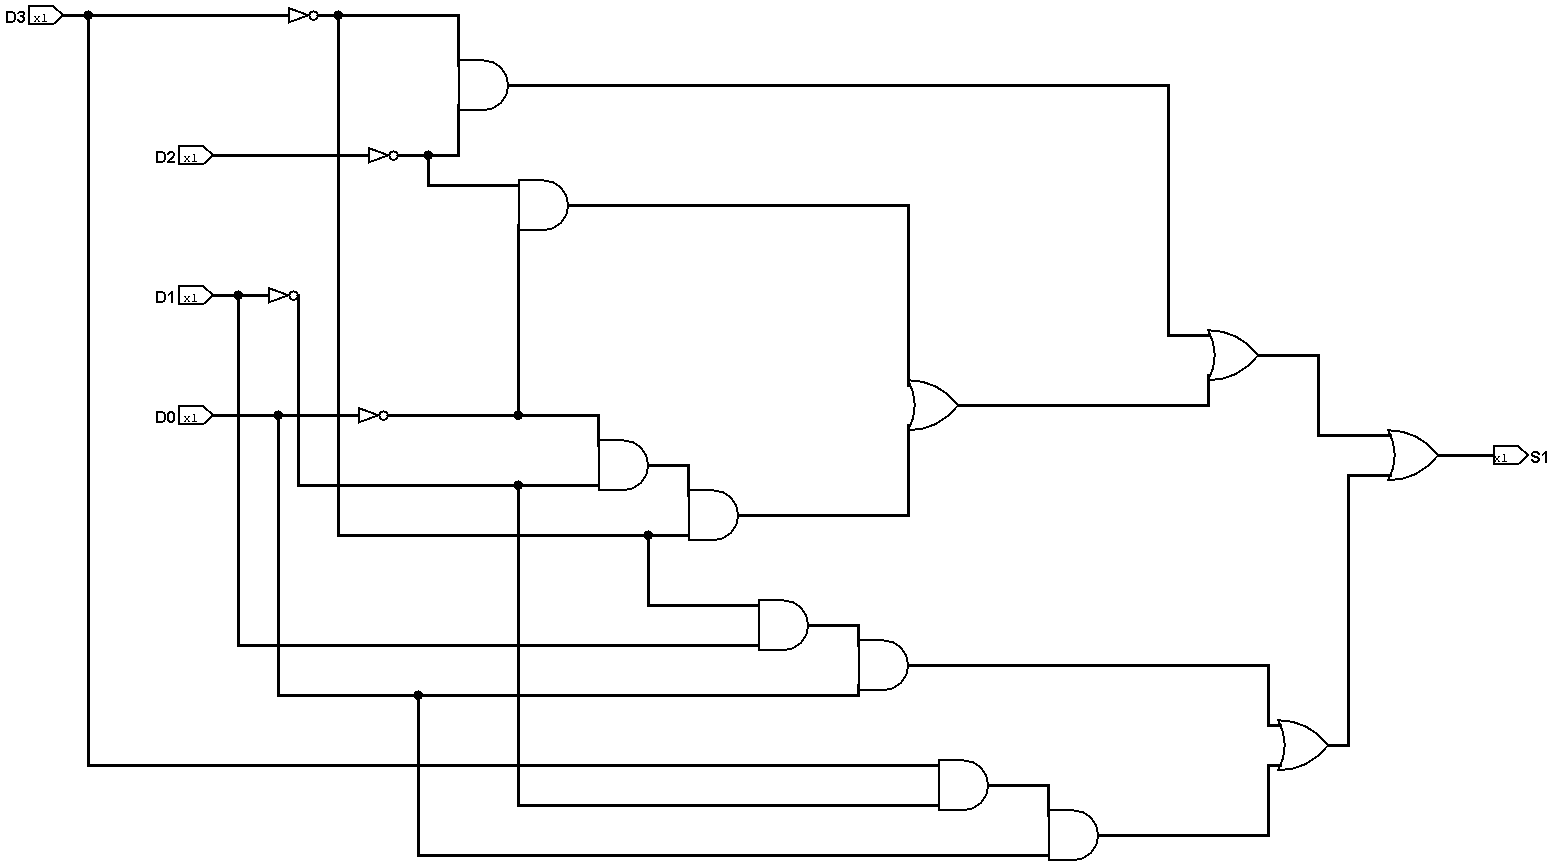
\includegraphics[width=0.7\textwidth]{part2_hex1.png}
    \caption{A schematic of HEX1}
    \label{f:part2_hex1}
\end{figure}

\begin{figure}[ht!]
    \centering
    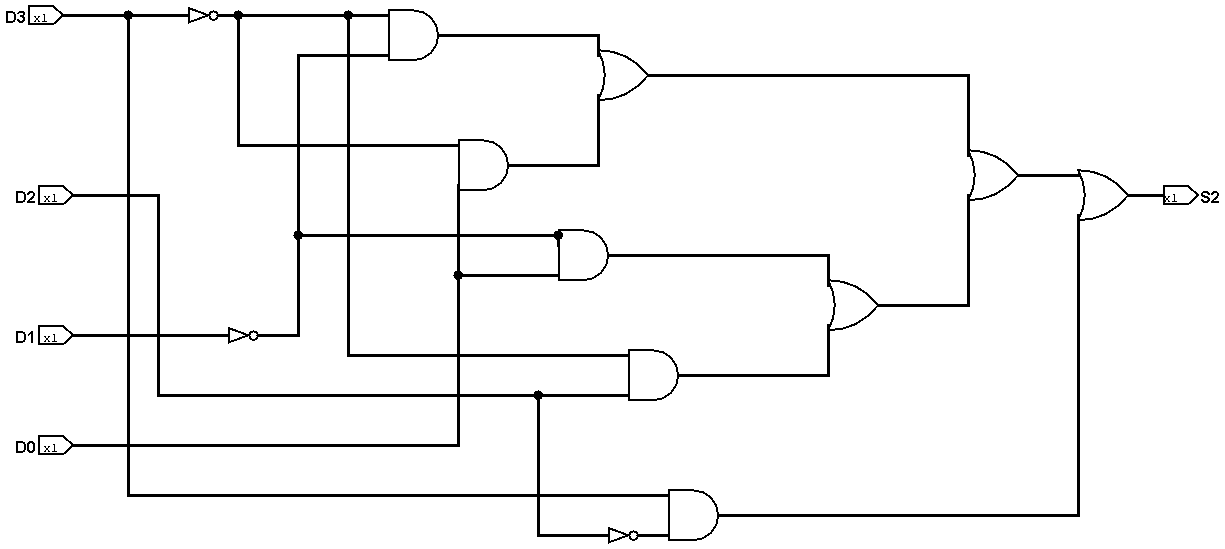
\includegraphics[width=0.7\textwidth]{part2_hex2.png}
    \caption{A schematic of HEX2}
    \label{f:part2_hex2}
\end{figure}


\begin{figure}[ht!]
    \centering
    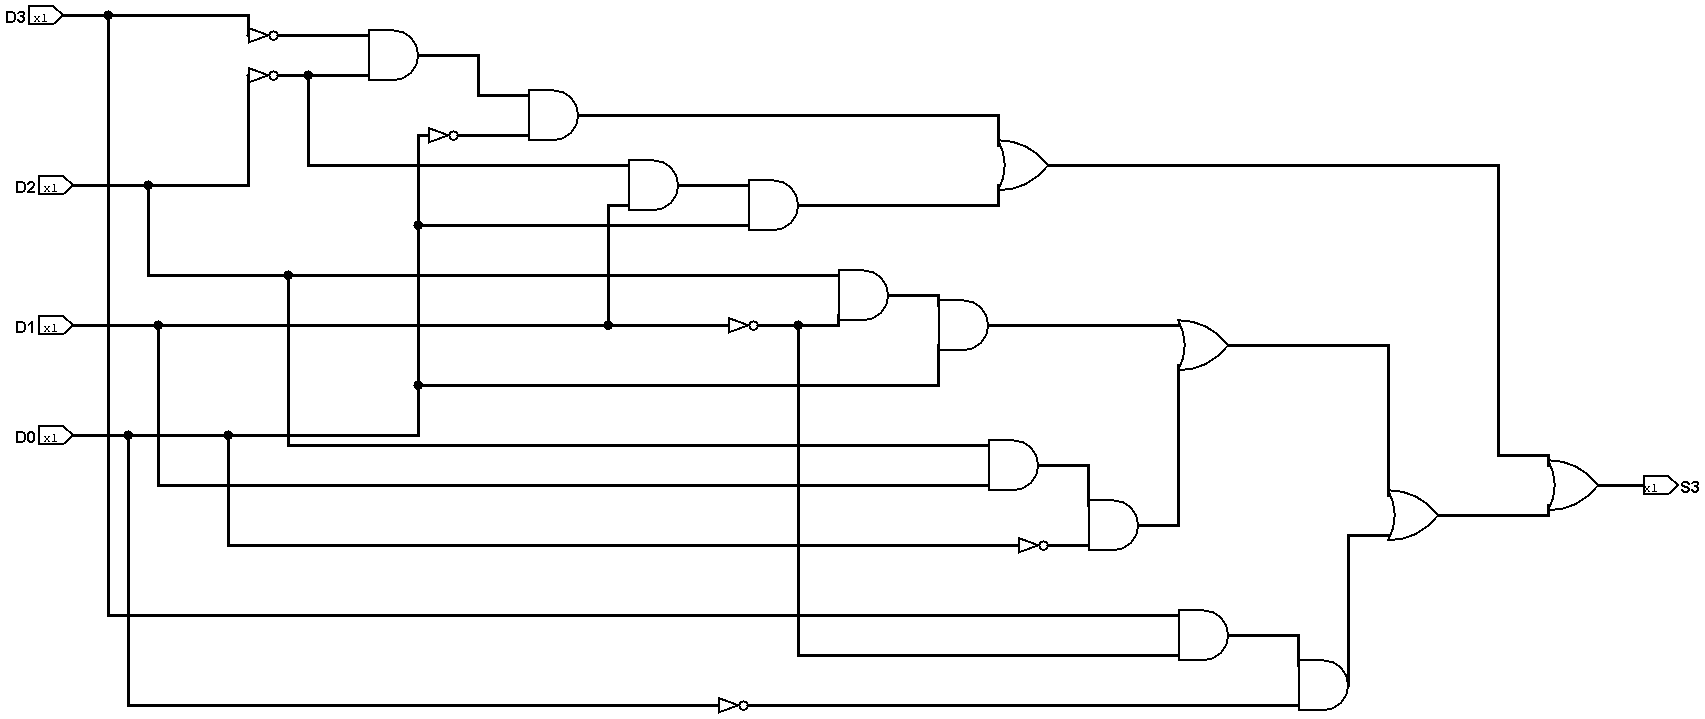
\includegraphics[width=0.7\textwidth]{part2_hex3.png}
    \caption{A schematic of HEX3}
    \label{f:part2_hex3}
\end{figure}

\begin{figure}[ht!]
    \centering
    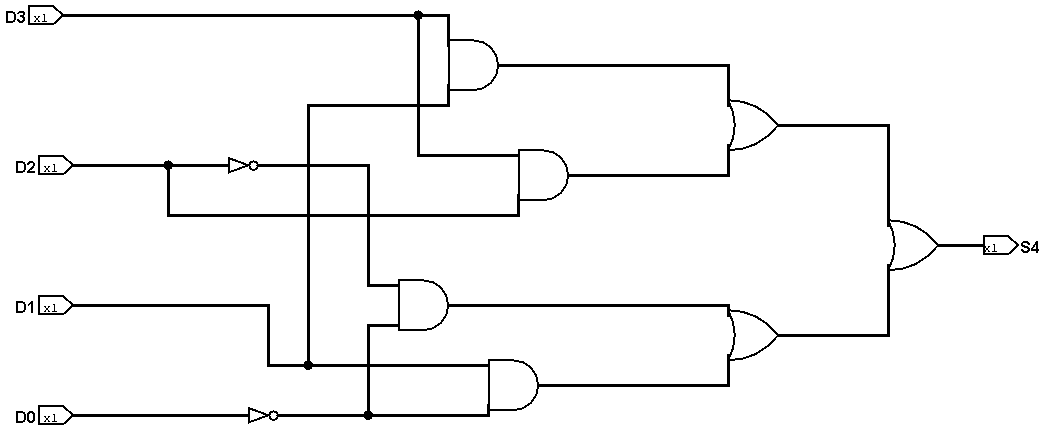
\includegraphics[width=0.7\textwidth]{part2_hex4.png}
    \caption{A schematic of HEX4}
    \label{f:part2_hex4}
\end{figure}

\begin{figure}[ht!]
    \centering
    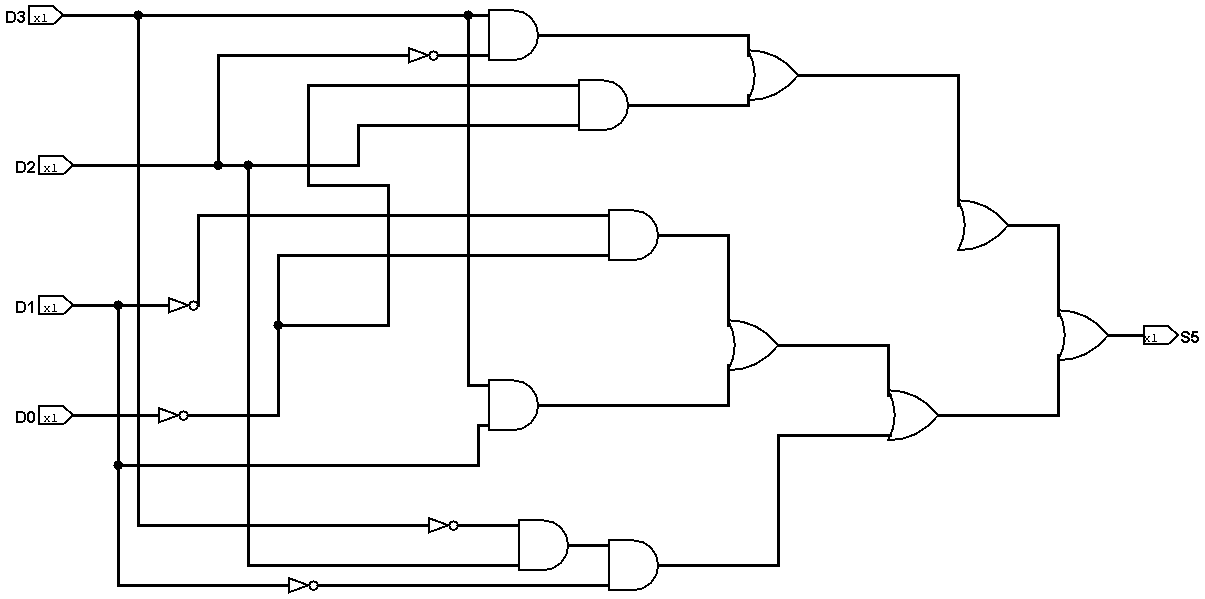
\includegraphics[width=0.7\textwidth]{part2_hex5.png}
    \caption{A schematic of HEX5}
    \label{f:part2_hex5}
\end{figure}

\begin{figure}[ht!]
    \centering
    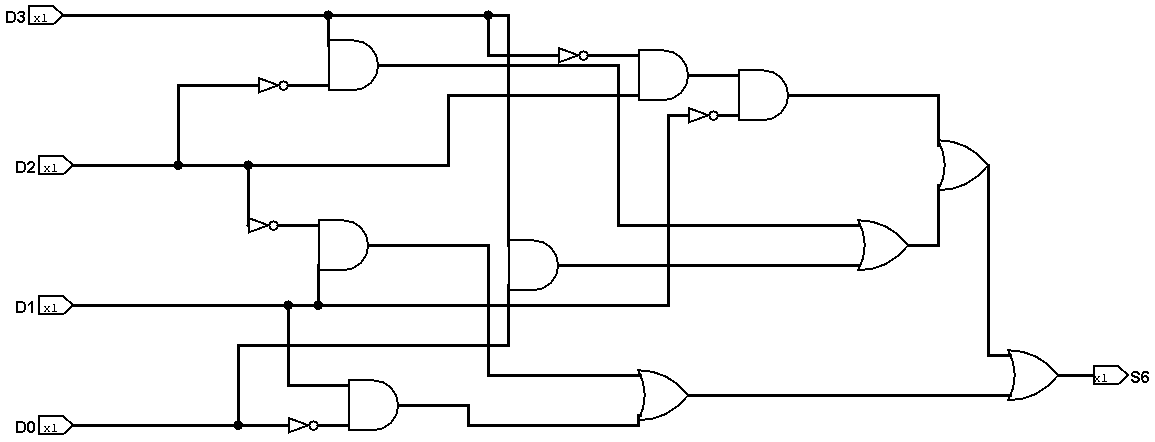
\includegraphics[width=0.7\textwidth]{part2_hex6.png}
    \caption{A schematic of HEX6}
    \label{f:part2_hex6}
\end{figure}

\end{enumerate}

\end{document}